\documentclass[acmsmall,screen]{acmart}

\setcopyright{none}
\settopmatter{printacmref=false}
\renewcommand\footnotetextcopyrightpermission[1]{}
\pagestyle{plain}

\usepackage{booktabs}
\usepackage{tabularx}
\usepackage{enumitem}
\usepackage{tikz}
\usetikzlibrary{arrows.meta,positioning,shapes.geometric,fit,backgrounds}

\title{Systematic Design of RAG-based LLM Inference Systems: A Survey}

\author{Repository Draft}
\affiliation{%
  \institution{Awesome-RAG-LLM-Inference-System Repository}
  \city{Online}
  \country{GitHub}
}

\begin{abstract}
Retrieval-augmented generation (RAG) has become a practical way to improve large language model (LLM) responses with external knowledge, but its deployment cost is increasingly shaped by systems concerns rather than model design alone. Modern RAG serving pipelines must coordinate query encoding, vector retrieval, reranking, prompt construction, and autoregressive decoding under tight latency, memory, and cost constraints. Recent work shows a clear shift from model-only optimization toward end-to-end co-design across accelerators, caches, schedulers, and storage systems. This survey organizes the repository literature into a unified taxonomy of RAG inference system design. We summarize the main system bottlenecks, review five major design axes, provide comparative discussion with explicit citations, and include framework figures for the end-to-end pipeline, the design taxonomy, and the memory hierarchy. The survey closes with cross-cutting trade-offs, research trends, and open challenges for building efficient, scalable, and quality-aware RAG inference systems.
\end{abstract}

\keywords{retrieval-augmented generation, large language models, inference systems, vector search, memory hierarchy, systems survey}

\begin{document}

\maketitle

\section{Introduction}

Retrieval-augmented generation has become a core architecture for knowledge-intensive LLM applications because it separates parametric generation from non-parametric knowledge storage. Instead of depending only on model weights, a RAG pipeline retrieves relevant external context, injects it into the prompt, and then decodes a response conditioned on both the query and the retrieved evidence. This design can improve factuality, freshness, domain adaptation, and controllability, but its practical value now depends heavily on end-to-end systems efficiency rather than retrieval quality alone.

The recent literature collected in this repository reflects a clear system-centric shift. End-to-end serving papers such as RAGO and Hermes treat RAG as a coordinated retrieval and generation pipeline rather than an isolated retrieval module~\cite{rago2025,hermes2025}. Cache-centric systems such as Cache-Craft, CacheBlend, MemoRAG, HyperRAG, CacheFocus, and METIS show that reuse, adaptation, and cache management increasingly determine both quality and cost~\cite{cachecraft2025,cacheblend2025,memorag2025,hyperrag2025,cachefocus2025,metis2025}. Scheduling-oriented work such as PipeRAG, RAGDoll, ELERAG, Patchwork, AquaPipe, and DGRAG demonstrates that overlap among retrieval, prompt construction, and decoding can be as important as speeding up any single stage~\cite{piperag2025,ragdoll2025,elerag2025,patchwork2025,aquapipe2025,dgrag2025}. Meanwhile, SmartSSD, near-data, and disk-native vector-search systems show that large-scale RAG cannot rely on GPU memory alone~\cite{smartssd2024,ndsearch2024,chameleon2025,diskann2019,lmdiskann2023,lsmvec2025}.

This survey provides a system-oriented synthesis of that design space. Our contributions are:
\begin{enumerate}[leftmargin=*]
  \item a taxonomy of RAG inference system designs spanning GPU acceleration, reuse, scheduling, external memory, and application-specific optimization;
  \item a comparison of architectural trade-offs across latency, throughput, memory capacity, quality, and freshness; and
  \item a summary of research trends and open challenges for scalable, efficient, and quality-aware RAG serving.
\end{enumerate}

\section{Background: RAG Inference as a Systems Pipeline}

An end-to-end RAG inference pipeline usually contains five stages: query encoding, vector retrieval, reranking or filtering, prompt construction, and LLM decoding. Although that decomposition is conceptually simple, each stage stresses a different part of the underlying system stack. Figure~\ref{fig:pipeline} illustrates the typical pipeline and the main bottlenecks exposed at each stage.

\begin{figure}[t]
\centering
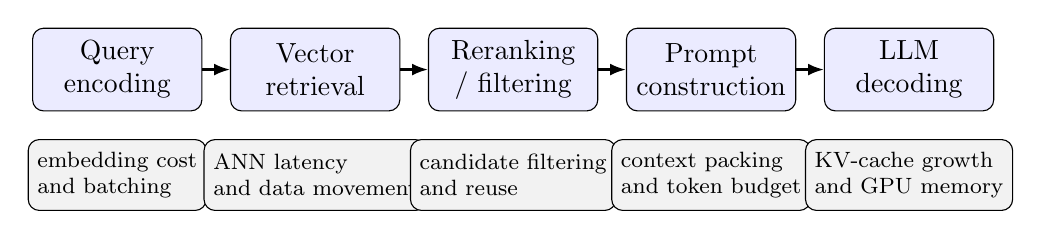
\begin{tikzpicture}[
  stage/.style={draw, rounded corners, align=center, minimum width=2.15cm, minimum height=1.05cm, fill=blue!8},
  note/.style={draw, rounded corners, align=left, minimum width=2.15cm, minimum height=0.9cm, fill=gray!10, font=\footnotesize},
  arr/.style={-{Latex[length=2mm]}, thick}
]
\node[stage] (q) {Query\\encoding};
\node[stage, right=0.35cm of q] (r) {Vector\\retrieval};
\node[stage, right=0.35cm of r] (rr) {Reranking\\/\ filtering};
\node[stage, right=0.35cm of rr] (p) {Prompt\\construction};
\node[stage, right=0.35cm of p] (d) {LLM\\decoding};

\draw[arr] (q) -- (r);
\draw[arr] (r) -- (rr);
\draw[arr] (rr) -- (p);
\draw[arr] (p) -- (d);

\node[note, below=0.35cm of q] {embedding cost\\and batching};
\node[note, below=0.35cm of r] {ANN latency\\and data movement};
\node[note, below=0.35cm of rr] {candidate filtering\\and reuse};
\node[note, below=0.35cm of p] {context packing\\and token budget};
\node[note, below=0.35cm of d] {KV-cache growth\\and GPU memory};
\end{tikzpicture}
\caption{A typical RAG inference pipeline. Practical serving stacks must coordinate retrieval-side latency, prompt-side orchestration, and decode-side memory pressure rather than optimizing only one stage.}
\Description{A five-stage pipeline diagram with boxes labeled query encoding, vector retrieval, reranking or filtering, prompt construction, and LLM decoding. A note below each box highlights its dominant system bottleneck.}
\label{fig:pipeline}
\end{figure}

\subsection{Latency, memory, and throughput bottlenecks}

Vector search can dominate latency when the corpus is large or when the index does not fit in fast memory. That pressure is visible in GPU-native search designs such as CAGRA, PilotANN, and VecFlow, which attempt to improve retrieval efficiency through accelerator-aware data structures and kernels~\cite{cagra2024,pilotann2025,vecflow2026}. In end-to-end RAG systems, however, retrieval is only one part of the path. RAGO and Hermes show that CPU/GPU transfers, scheduling gaps, and prompt assembly overhead can materially affect end-to-end performance even when the underlying ANN component is fast~\cite{rago2025,hermes2025}.

Memory is the second persistent bottleneck. RAG serving must simultaneously manage vector indexes, retrieved context, and expanding LLM KV caches. As corpora and context windows grow, accelerator memory becomes insufficient, which motivates disaggregated and hierarchical memory designs such as Chameleon, SmartSSD-based search, DiskANN, and LSM-VEC~\cite{smartssd2024,chameleon2025,diskann2019,lsmvec2025}. Throughput is the third bottleneck: if retrieval, reranking, and decoding have mismatched service rates, queues accumulate and hardware remains underutilized~\cite{piperag2025,patchwork2025,aquapipe2025}.

\subsection{Key evaluation metrics}

A complete RAG-system evaluation should include average latency, tail latency, throughput under concurrency, answer quality or recall, memory footprint, cost efficiency, and freshness support. Recent work has also made energy efficiency and quality-aware control more visible, especially for hardware-specialized or adaptive systems~\cite{metis2025,ndsearch2024,smartssd2024}. These metrics motivate the taxonomy in Figure~\ref{fig:taxonomy}.

\begin{figure}[t]
\centering
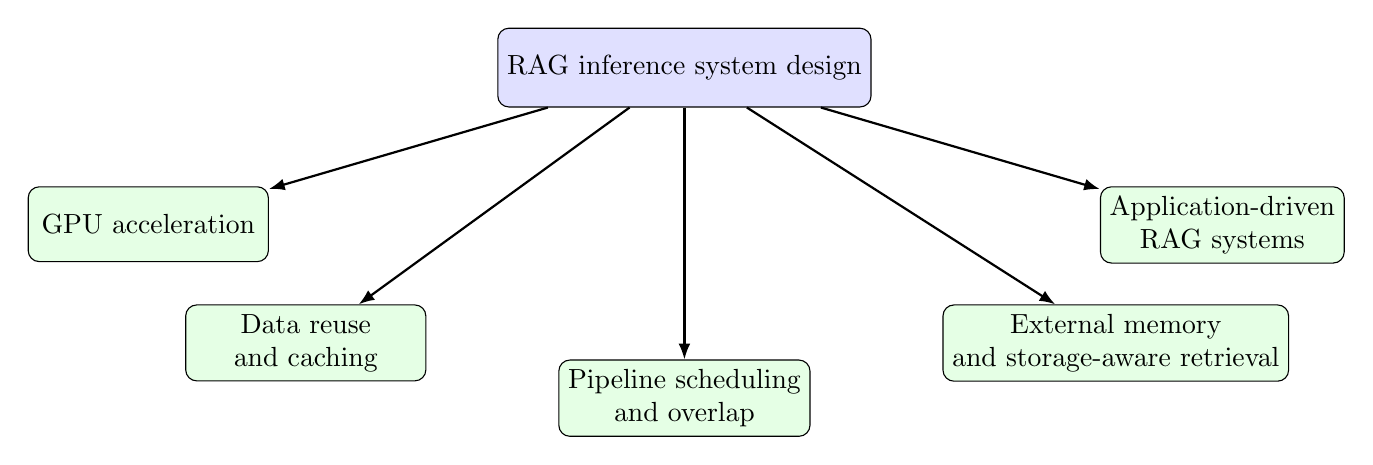
\begin{tikzpicture}[
  root/.style={draw, rounded corners, fill=blue!12, align=center, minimum width=4.2cm, minimum height=1cm},
  leaf/.style={draw, rounded corners, fill=green!10, align=center, minimum width=3.05cm, minimum height=0.95cm},
  arr/.style={-{Latex[length=2mm]}, thick}
]
\node[root] (root) {RAG inference system design};
\node[leaf, below left=1.0cm and 2.9cm of root] (gpu) {GPU acceleration};
\node[leaf, below left=2.5cm and 0.9cm of root] (cache) {Data reuse\\and caching};
\node[leaf, below=3.2cm of root] (sched) {Pipeline scheduling\\and overlap};
\node[leaf, below right=2.5cm and 0.9cm of root] (mem) {External memory\\and storage-aware retrieval};
\node[leaf, below right=1.0cm and 2.9cm of root] (app) {Application-driven\\RAG systems};
\draw[arr] (root) -- (gpu);
\draw[arr] (root) -- (cache);
\draw[arr] (root) -- (sched);
\draw[arr] (root) -- (mem);
\draw[arr] (root) -- (app);
\end{tikzpicture}
\caption{Taxonomy used in this survey. The current literature clusters around accelerator-aware retrieval, reuse-centric serving, scheduling and pipelining, memory-hierarchy expansion, and workload-specific system design.}
\Description{A taxonomy tree with a root node labeled RAG inference system design and five child nodes labeled GPU acceleration, data reuse and caching, pipeline scheduling and overlap, external memory and storage-aware retrieval, and application-driven RAG systems.}
\label{fig:taxonomy}
\end{figure}

\section{Taxonomy of RAG Inference System Design}

\subsection{GPU acceleration}

The first line of work adapts vector search and end-to-end RAG serving to GPU architectures. Systems such as RAGO and Hermes illustrate the end-to-end view: retrieval, data movement, prompt handling, and generation are jointly optimized around the accelerator~\cite{rago2025,hermes2025}. At the algorithm level, CAGRA, PilotANN, and VecFlow show how GPU-oriented graph search, partitioning, and filtered vector data management can increase parallelism and reduce memory stalls~\cite{cagra2024,pilotann2025,vecflow2026}. Related CPU/GPU collaborative designs highlight that hybrid placement remains attractive when the retrieval corpus is large or when preliminary filtering can reduce accelerator load~\cite{cpugpucollab2025}.

Three themes recur in this category. First, GPU-native data structures often outperform CPU-derived designs once search order, graph layout, and memory access patterns are reorganized for SIMT execution~\cite{cagra2024}. Second, end-to-end overlap matters: a fast retrieval kernel does not automatically yield a fast RAG service if transfers and prompt orchestration remain serialized~\cite{rago2025,hermes2025}. Third, accelerator capacity remains the main limitation, which naturally motivates cache reuse and external memory.

\subsection{Data reuse and cache-centric optimization}

The second design axis treats reuse as a primary systems strategy. Cache-Craft and CacheBlend focus on knowledge reuse directly within the serving stack, showing that repeated access to documents or fused cached knowledge can substantially reduce end-to-end latency~\cite{cachecraft2025,cacheblend2025}. MemoRAG and HyperRAG extend this view by reusing memory summaries and reranker KV caches to improve quality-efficiency trade-offs in long-context or reranking-heavy settings~\cite{memorag2025,hyperrag2025}. CacheFocus and METIS demonstrate that static caches are often insufficient: efficient RAG systems increasingly need dynamic repositioning and quality-aware configuration control~\cite{cachefocus2025,metis2025}.

This literature spans several reuse targets: retrieved evidence, prompt-side context, reranker states, decoder KV caches, and operating configurations. The shared insight is that many workloads exhibit temporal or semantic locality. Yet reuse must be balanced against freshness and storage cost. EdgeRAG and SPFresh, for example, highlight the importance of online updates and evolving indexes when the knowledge base changes over time~\cite{edgerag2024,spfresh2023}. As a result, caching is no longer a minor optimization; it is becoming a first-class architectural component of RAG serving.

\subsection{Pipeline parallelism and scheduling}

The third line of work studies how retrieval and generation interact in time. PipeRAG, RAGDoll, ELERAG, AquaPipe, Patchwork, and DGRAG all show that overlapping retrieval, prompt construction, and decoding can significantly improve user-visible performance~\cite{piperag2025,ragdoll2025,elerag2025,aquapipe2025,patchwork2025,dgrag2025}. Some systems rely on adaptive pipelining, some on offloading, and some on lookahead retrieval or distributed placement, but they all emphasize orchestration rather than isolated component speed.

This category also reveals the limits of naive overlap. Retrieval difficulty varies from query to query; speculative retrieval can waste work; and heterogeneous systems are harder to balance under changing load~\cite{piperag2025,elerag2025,dgrag2025}. Even so, the broader lesson is important: queueing behavior, overlap, and resource assignment can influence end-to-end latency as much as the underlying ANN algorithm.

\subsection{External-memory and storage-aware acceleration}

Large-scale RAG frequently exceeds the memory budget of a single accelerator or server. The fourth axis therefore studies how to push computation closer to storage or how to extend the effective memory hierarchy beyond GPU HBM and CPU DRAM. Figure~\ref{fig:memory-hierarchy} illustrates the hierarchy emphasized by this literature.

\begin{figure}[t]
\centering
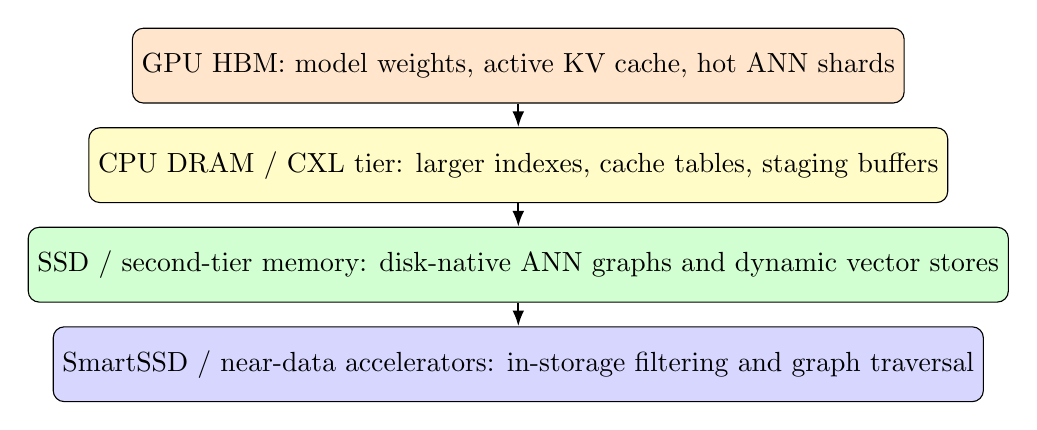
\begin{tikzpicture}[
  tier/.style={draw, rounded corners, minimum width=8.0cm, minimum height=0.95cm, align=center},
  arr/.style={-{Latex[length=2mm]}, thick}
]
\node[tier, fill=orange!20] (hbm) {GPU HBM: model weights, active KV cache, hot ANN shards};
\node[tier, fill=yellow!22, below=0.3cm of hbm] (dram) {CPU DRAM / CXL tier: larger indexes, cache tables, staging buffers};
\node[tier, fill=green!18, below=0.3cm of dram] (ssd) {SSD / second-tier memory: disk-native ANN graphs and dynamic vector stores};
\node[tier, fill=blue!16, below=0.3cm of ssd] (smart) {SmartSSD / near-data accelerators: in-storage filtering and graph traversal};
\draw[arr] (hbm) -- (dram);
\draw[arr] (dram) -- (ssd);
\draw[arr] (ssd) -- (smart);
\end{tikzpicture}
\caption{Memory hierarchy for large-scale RAG inference. Current systems increasingly span accelerator memory, host memory, second-tier memory, SSD-resident indexes, and near-data processing.}
\Description{A layered memory-hierarchy diagram with four horizontal tiers labeled GPU HBM, CPU DRAM or CXL tier, SSD or second-tier memory, and SmartSSD or near-data accelerators. Arrows connect the tiers from top to bottom.}
\label{fig:memory-hierarchy}
\end{figure}

\subsubsection{Processing in memory and near-data processing}

SmartSSD-based search, NDSEARCH, and Chameleon represent a strong trend toward reducing data movement for vector search and retrieval-heavy RAG deployments~\cite{smartssd2024,ndsearch2024,chameleon2025}. These systems move filtering, graph traversal, or search acceleration closer to storage or specialized hardware, which can improve scalability and sometimes energy efficiency. The trade-off is platform specificity: the systems are effective, but often require custom runtimes, hardware assumptions, or co-designed index layouts.

\subsubsection{Second-tier memory and disk-resident vector search}

DiskANN, LM-DiskANN, FreshDiskANN, and LSM-VEC show how disk-native or second-tier-memory-aware index structures can maintain large searchable corpora without requiring everything to remain in DRAM or GPU memory~\cite{diskann2019,lmdiskann2023,freshdiskann2021,lsmvec2025}. Their main value is scalability at low memory cost, while their main risk is I/O sensitivity. For production RAG, this trade-off is increasingly acceptable because the knowledge store is often too large or too dynamic for fully in-memory operation.

\subsection{Application-driven RAG systems}

The final category focuses on applications whose domain constraints reshape system design. SEFRQO applies RAG to query optimization, where the retrieved objects and utility function differ from open-domain text generation~\cite{sefrqo2026}. AixelAsk targets table question answering and demonstrates how structured data and stepwise reasoning change retrieval patterns and prompt construction needs~\cite{aixelask2026}. These cases suggest that future RAG platforms will need flexible abstractions that support workload-specific indexing, caching, and scheduling choices rather than a single universal architecture.

\section{Cross-cutting Design Dimensions}

\subsection{Latency versus quality}

Approximate retrieval, aggressive caching, and lookahead scheduling can reduce latency, but each may risk lower recall or worse answer quality. Quality-aware systems such as METIS and AquaPipe are notable because they expose this trade-off directly rather than assuming that the fastest execution path is always acceptable~\cite{metis2025,aquapipe2025}. A mature RAG-serving stack should select operating points based on service-level objectives and quality targets.

\subsection{Throughput versus memory capacity}

Higher throughput often requires more memory for larger GPU-resident indexes, pipeline buffers, or caches. Yet keeping everything in fast memory is frequently impossible. This tension explains the rise of heterogeneous designs that combine GPUs, CPUs, CXL-like expansion, SSDs, and near-data accelerators~\cite{chameleon2025,diskann2019,smartssd2024}. Memory hierarchy management is therefore central rather than peripheral.

\subsection{Static indexing versus dynamic updates}

Production knowledge bases change continuously. Efficient support for online updates remains difficult because caches, vector indexes, and storage layouts all need to adapt together. SPFresh, EdgeRAG, FreshDiskANN, and LSM-VEC indicate that freshness support is becoming a central requirement for production-scale RAG systems~\cite{spfresh2023,edgerag2024,freshdiskann2021,lsmvec2025}.

\subsection{Monolithic versus heterogeneous architectures}

Some systems target tightly integrated single-node performance, while others distribute work across CPUs, GPUs, storage devices, or edge-cloud deployments. Heterogeneous architectures can scale further and use memory more efficiently, but they increase scheduling complexity and widen the operating-design space~\cite{ragdoll2025,dgrag2025,chameleon2025}. The best architecture depends strongly on workload and deployment constraints.

\subsection{Retrieval-centric versus generation-centric optimization}

Many papers begin from either the ANN side or the LLM serving side, but the strongest recent systems increasingly optimize both together. RAGO, Hermes, Patchwork, and HyperRAG all emphasize that chunk selection, prompt assembly, cache reuse, and decode-time scheduling interact in ways that make stage-local optimization insufficient~\cite{rago2025,hermes2025,patchwork2025,hyperrag2025}.

\section{Comparative View of Representative Systems}

Table~\ref{tab:comparison} summarizes representative systems from the repository and highlights their main optimization targets and trade-offs.

\begin{table*}[t]
\caption{Representative systems and their primary design trade-offs.}
\label{tab:comparison}
\footnotesize
\begin{tabularx}{\textwidth}{@{}p{1.6cm}p{0.8cm}p{2.1cm}p{2.0cm}p{1.8cm}p{2.2cm}X@{}}
\toprule
Paper & Year & Main target & Optimization level & Hardware setting & Main benefit & Key trade-off \\
\midrule
RAGO~\cite{rago2025} & 2025 & End-to-end RAG serving & System pipeline & GPU & Lower latency and higher throughput & Additional orchestration complexity \\
Hermes~\cite{hermes2025} & 2025 & Efficient large-scale RAG & Algorithm--system co-design & GPU & Better accelerator utilization & GPU-memory dependence \\
CAGRA~\cite{cagra2024} & 2024 & GPU ANN search & Index and kernel design & GPU & High parallel vector search & Limited by accelerator capacity \\
Cache-Craft~\cite{cachecraft2025} & 2025 & Chunk-cache management & Cache reuse & CPU/GPU serving & Fewer repeated retrievals & Freshness and cache sizing \\
CacheBlend~\cite{cacheblend2025} & 2025 & Cached knowledge fusion & Model-serving reuse & GPU/LLM serving & Faster serving & Cache validity \\
MemoRAG~\cite{memorag2025} & 2025 & Long-context reuse & Memory-enhanced retrieval & Heterogeneous serving & Better context reuse & Added state-management overhead \\
METIS~\cite{metis2025} & 2025 & Quality-aware RAG & Adaptive control & Heterogeneous & Better quality-efficiency control & Controller complexity \\
PipeRAG~\cite{piperag2025} & 2025 & Adaptive pipelining & Scheduling & Heterogeneous & Retrieval-generation overlap & Backpressure and balancing \\
Patchwork~\cite{patchwork2025} & 2025 & Unified RAG serving & Framework design & Heterogeneous & Integrated end-to-end serving & Wider orchestration scope \\
SmartSSD search~\cite{smartssd2024} & 2024 & Billion-scale retrieval & Near-data processing & SmartSSD & Scalability beyond host memory & Hardware specialization \\
Chameleon~\cite{chameleon2025} & 2025 & Retrieval-augmented LMs & Disaggregated acceleration & Heterogeneous accelerators & Better memory scalability & Deployment complexity \\
DiskANN~\cite{diskann2019} & 2019 & Disk-native ANN & Index + I/O design & SSD & Large-scale low-memory search & I/O-sensitive performance \\
LSM-VEC~\cite{lsmvec2025} & 2025 & Dynamic vector search & Storage-aware updates & SSD + memory & Better update support at scale & More complex maintenance path \\
SEFRQO~\cite{sefrqo2026} & 2026 & Query optimization & Application-specific RAG & Database setting & Domain-aware retrieval benefits & Narrower workload scope \\
\bottomrule
\end{tabularx}
\end{table*}

The table highlights a broad trajectory in the literature. Earlier work often isolates a specific bottleneck such as GPU ANN search or disk-resident indexing, while newer systems combine ideas from caching, scheduling, and heterogeneous-memory management. This convergence suggests that future RAG platforms will increasingly resemble integrated data systems rather than loosely coupled model pipelines.

\section{Research Trends}

The repository literature suggests five major trends. First, RAG is becoming a systems problem rather than a retrieval-only problem~\cite{rago2025,hermes2025,patchwork2025}. Second, cache reuse is now a first-class design principle rather than a minor serving optimization~\cite{cachecraft2025,cacheblend2025,memorag2025,hyperrag2025}. Third, memory hierarchy management is central because GPU memory alone is insufficient for many realistic deployments~\cite{smartssd2024,chameleon2025,diskann2019}. Fourth, near-data and storage-aware acceleration are becoming practical for large retrieval-heavy workloads~\cite{ndsearch2024,smartssd2024,lsmvec2025}. Fifth, quality-aware adaptation is emerging as a necessary control layer for production systems that must balance speed and answer quality~\cite{metis2025,aquapipe2025}.

\section{Open Challenges and Future Directions}

Despite rapid progress, several problems remain open.
\begin{itemize}[leftmargin=*]
  \item \textbf{Unified evaluation methodology.} Different papers use different datasets, retrieval settings, concurrency assumptions, and quality metrics, which makes direct comparison difficult.
  \item \textbf{Joint optimization of retrieval and decoding.} Many systems still optimize retrieval and generation separately, even though chunk selection, prompt packing, and decode scheduling interact strongly~\cite{rago2025,hyperrag2025,patchwork2025}.
  \item \textbf{Dynamic and continuously updated knowledge bases.} Freshness support remains difficult once caches, indexes, and storage layouts must all evolve together~\cite{spfresh2023,edgerag2024,lsmvec2025}.
  \item \textbf{Long-context and memory-intensive RAG.} Larger contexts amplify prompt assembly cost and KV-cache pressure, pushing future systems toward compression, reuse, and richer memory hierarchies~\cite{memorag2025,chameleon2025}.
  \item \textbf{Multi-tenant production serving.} Tenant isolation, cost-aware scheduling, and service-level management remain underexplored despite their practical importance.
  \item \textbf{Application-specific architectures.} Query optimization, table reasoning, coding assistance, enterprise QA, and edge deployment may each require different retrieval and serving abstractions~\cite{sefrqo2026,aixelask2026,dgrag2025}.
\end{itemize}

\section{Conclusion}

RAG-based LLM inference has evolved into a rich systems research area. Efficient deployment depends on much more than retrieval accuracy: GPU-native vector search, cache-centric optimization, pipeline scheduling, external-memory support, and application-aware design all shape the final latency, throughput, quality, and cost of a service. The literature collected in this repository makes one point especially clear: future RAG systems will be won by co-design across retrieval, generation, memory hierarchy, and orchestration. That integrated perspective is the central takeaway of this survey.

\bibliographystyle{ACM-Reference-Format}
\bibliography{references}

\end{document}
